\documentclass[10pt,jaurnal,compsoc]{IEEEtran}

\usepackage[pdftex]{graphicx}
\usepackage{cite}
\hyphenation{op-tical net-works semi-conduc-tor}


\begin{document}

\title{Using Deep Neural Networks for autonomus drone navigation in orchard enviroiment}

\author{BRESILLA, Trim}

\markboth{Inference project, Robotic Nanodegree, Udacity}%
{}
\IEEEtitleabstractindextext{%

\begin{abstract}
    With the increase of population in the world, the demand for quality food is increasing too. One of the biggest and the base of raw food production comes frim Agriculture. In the recent years, due to this demand, and other enviroimental factors have havily influenced the way agricultural production is done. Automation and robotics for fruit and vegetable production and monitoring has become the new standard. In this /paper/ we disscus an autonomus drone that would be bale to navigate through the rows in an onrchard enviroiment. The drone is made of a flight controller (PixHawk), an micorocntroller (Aarduino) for analog reading from differnet sensors, and a on-board computer (Raspberry Pi gen. 3). Pictres are taken through PiCamera and streamed through WiFi to a computer running a neaurl network model. Based on prior trainings, the moderunning a neaurl network model. Based on prior trainings, the model sents back the direction to the drone, thus performing navigation.
\end{abstract}

\begin{IEEEkeywords}
Robotics, Agriculture, Udacity, Orchard, Deep Learning.
\end{IEEEkeywords}}


\maketitle
\IEEEdisplaynontitleabstractindextext
\IEEEpeerreviewmaketitle
\section{Introduction}↓
\label{sec:introduction}

\IEEEPARstart{A}{utomation} in Agriculture is recent years i highly increasing. Eventhough Agriculture as one of the oldest occupation in the world, has seen many changes during centuries. Before Industrial Revolution was estimated that more than 80\% of population were working as farmers, while now is estimated that number to be 2\%. One of the dominant changes that characteries a growing economy is the proportionate decline in Agriculture Sector. This phenomenon is commonly atributed to two facts: food is not as demnading as other goods and services, and the rapid development of new farming technologies lead to expanding food supplies per hectare and per worker.
%IMAGE
\begin{figure}[thpb]
      \centering
      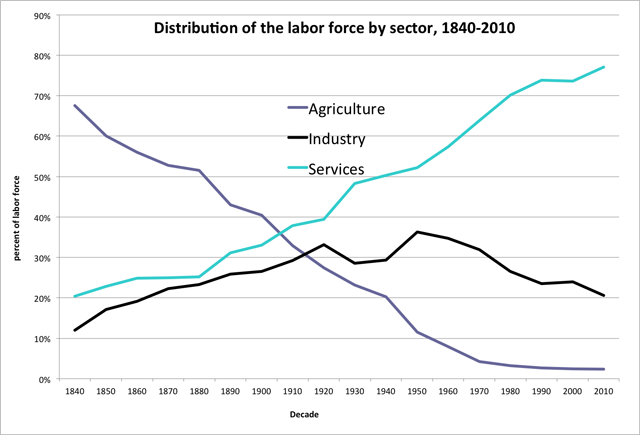
\includegraphics[width=\linewidth]{agridecline}
      \caption{Industrial Revolution.}
      \label{fig:robot1}
\end{figure}

The decrease shows significance every step of the industrial revolution. Industry 1.0 brought mechanisation, water management etc.; Industry 2.0 brought steam engines, electricity, protected enviroiments etc.; Industry 3.0 broight computers and smart apliances, GPS trctors and so on; while Industry 4.0 is foreseen to be the most significant one, bringing AI, Automation and Robotics.

The chanllenge of how we'll feed the evergrowing world populatoin in the future - is sustainable, cost-effective anf most importantly enviroimentally friendly. In order to feed 9.5 billion people that Food and Agriculture Organisation (FAO) predicts to inhabit the planet by 2050 while climate change is making more dificult to grow crops - is going to be done by Smart Farming, a high-tech and AI driven agricultural management system. Agriculture is highly repetitive, and such, many tasks can and are being automated. Individual agricultural activities on the farm takes effort, for example planting, maintaining, and harvesting crops need money, energy, labor and resources. What if we can use technology to replace some of the human activities and guarantee efficiency? That’s where artificial intelligence comes in. Agriculture is slowly becoming digital and AI in agriculture is emerging in three major categories, (i) agricultural robotics, (ii) soil and crop monitoring, and (iii) predictive analytics.

For a farmer robot to be fully autonomus, it needs to navigate through quiet diverse and harsh enviroiment without the human supervision, then perform a set of actions at specific location like: pickin a fruit, evalute a site, spray pesticide, cut branches, plant a seed, image and scan a whole plant and take specified measurement. Controlled enviroiments like greenhouses are more managable because of controllable enviroment and better engineered, where the sensor measurements produce less nois. Whereas outdoor environment are much harsher and generaly not controllable, thus making far more difficult than indoor enviroiments. Most of outdoor robot are equiped with GPS for sensing the location, but due to accuracy, they are often companioned with other sensors like IMUs, 3DCameras, Rotary Encoders to create a sensor fusuin for a much precise action taking proces. Robots nowadays are wirelessly connected to a central operator to both receive updated instructions regarding the mission, and report status and data. However, making an autonomous farm robot requires clever controllers, localisation, communication and actioin taking systems. The technology is similar to that of autonomous cars applied to agtech. Where it differs is that farming robots often need to manipulate their environment, picking vegetables or fruits, applying pesticides in a localised manner, or planting seeds. All these tasks require sensing, manipulation, and processing of their own.

In fruit production, as is with all other fields of agriculture, crop monitoring is extremely important as there can be estimation ahead of time thus making to the farmer vere easy to pln logistics anddistributions. In this paper is discussed an autonous Unmanned Areal Vehicle (UAV) flying under tree canapy, between two rows and under the anti-hail nets. In order for the robot to sucessfully follow the the row, it has firsly to know the orchard and where is the startig row, then has to percie the path between two rows while maintaining the altitude and avoind any collision with lateral branches fo the trees and void any other obsacles. 

\section{Background / Formulation}

\section{Data Acquisition}

\section{Results}

\section{Discussion}

\section{Conclusion / Future work}

\bibliography{bib}
\bibliographystyle{ieeetr}

\end{document}
